%TEX root = ../dissertation.tex

\chapter{Implementation}
\label{chapter:implementation}

For our Pulsarcast implementation we decided to take advantage of the
\emph{libp2p} ecosystem as it solves a lot of the underlying issues of building
a peer to peer system, not specific to our pubsub scenario. This includes
dealing with connection multiplexing, NAT traversal, discovery mechanisms, etc.
All of which libp2p, a community focused project with implementations in
multiple languages already solves. We can also take advantage of the utility
modules it has and the advantage of having an already working implementation of
the Kadmelia DHT. Our focus is then to build a module, implementing the
Pulsarcast specification, that clients and apps can take advantage of. Section
\ref{pulsarcast-javascript-module} provides a detailed description of it.

Besides our module, we also needed to find a suitable way to test our system as
whole. Given our specific needs, we opted to build a custom testbed, detailed
in section \ref{testbed} and the basis of the evaluation detailed in chapter
\ref{chapter:evaluation}. 

\section{Pulscarcast Javascript module}\label{pulsarcast-javascript-module}

We chose to implement our Pulsarcast module in Javascript. As it was covered in
our related work, Javascript is ubiquitous, running in browsers, servers and
many different kinds of devices and architectures. Through it, we are able to
run our Pulscarcast nodes in a multitude of systems and most importantly,
direct its usage for the World Wide Web. Plus, libp2p has a Javascript
implementation focused on cross compatibility between server and browser. This
is not to say that in the future we will not have other implementations in
different languages, that is in fact one of the reasons for the clear
separation between the Pulcarcast specification and its actual implementation.
However, we had to choose, and in our view Javascript is the clear winner. It is worth noting that, much like the work we built on top of, this module is open source~\footnote{https://github.com/JGAntunes/js-pulsarcast}.

\subsection{Dependencies}\label{subsec:dependencies}

Figure \ref{fig:pulsarcast-in-libp2p} gives us an overview of how our module
fits in the libp2p ecosystem. libp2p defines interfaces responsible for routing
content (peer routing), discovering other peers in the network (peer
discovery), network transports and leveraging multiple network connections
(switch). These all come bundled in the libp2p javascript
module~\footnote{https://github.com/libp2p/js-libp2} which we use in
Pulsarcast. Besides the main libp2p module we also use some other utility
modules such as the CID
module~\footnote{https://github.com/multiformats/js-cid} and the Peer-id
module~\footnote{https://github.com/libp2p/js-peer-id}, both designed to reason
with content identifiers (peer identifiers are also content identifiers). 

\begin{figure}[hb!]
  \centering
  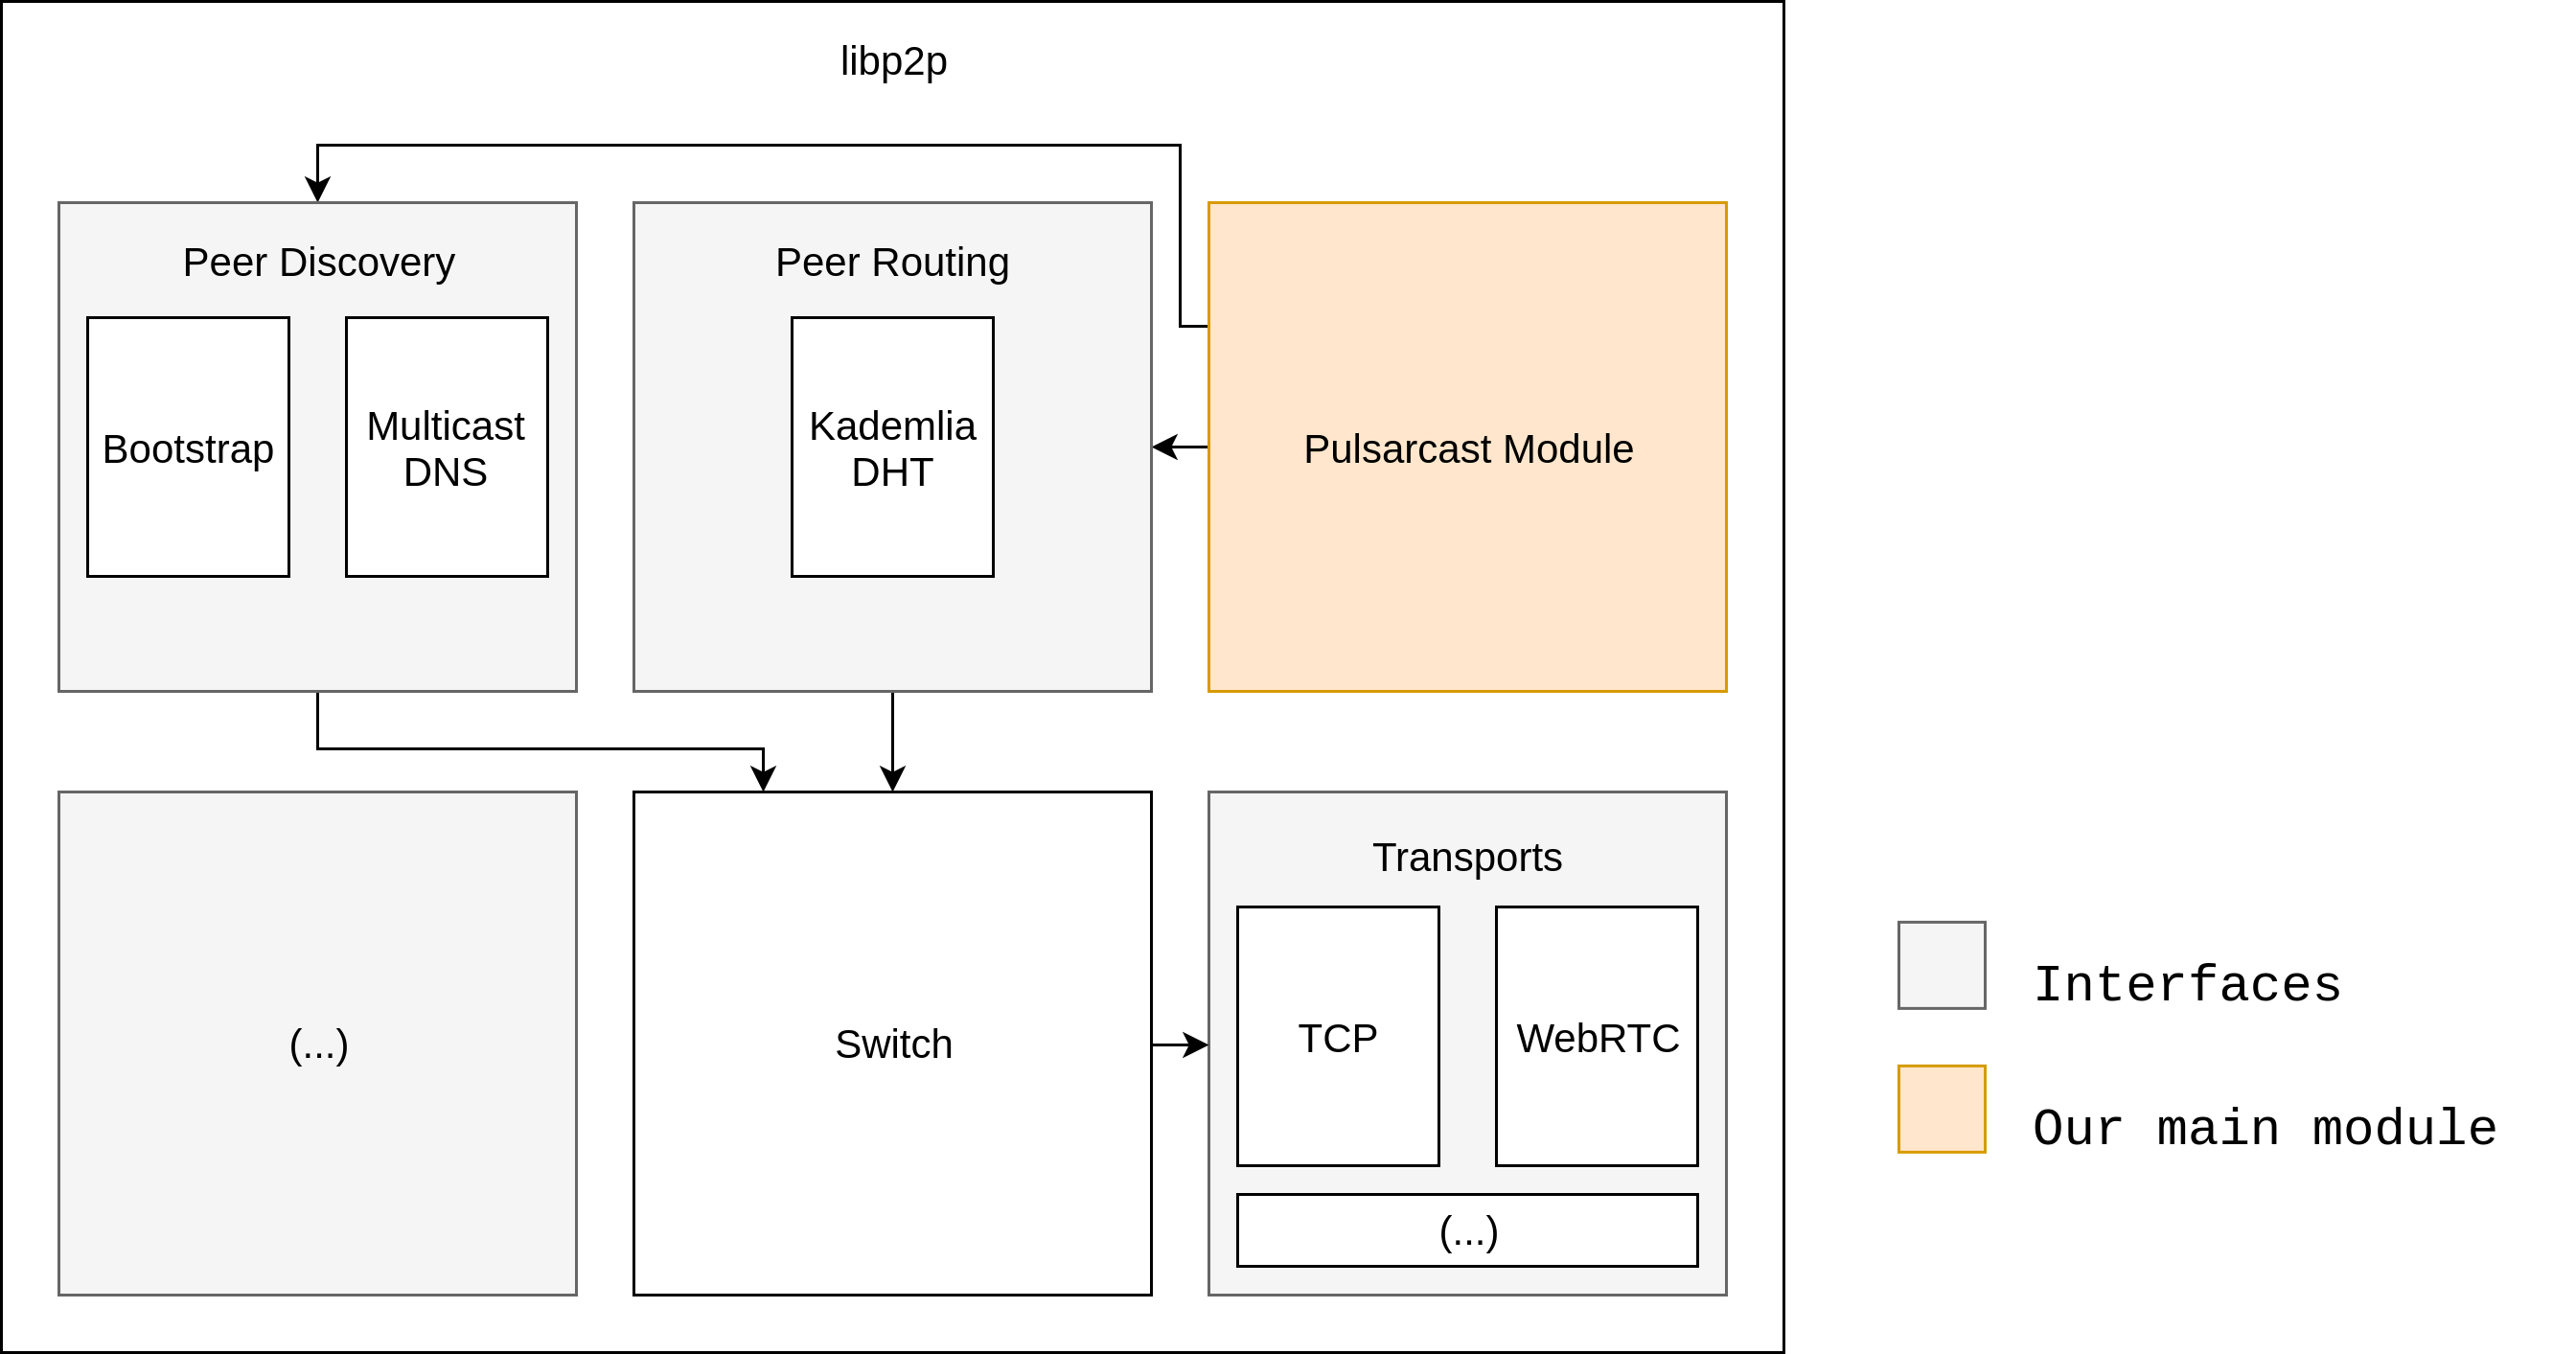
\includegraphics[width=0.95\textwidth]{img/pulsarcast-in-libp2p.png}
  \caption{Our Pulsarcast module in the libp2p ecosystem}
  \label{fig:pulsarcast-in-libp2p}
\end{figure}

Other than the libp2p dependencies, we have used other open source community
modules. The listing \ref{dependencies} shows our dependency list, pulled from
our \emph{package.json} (our module manifest). We have used a couple of helpers
for handling data streams~\footnote{https://github.com/pull-stream/pull-stream}
as well as a library to help us with the asynchronous control
flow~\footnote{https://github.com/caolan/async}. To help us with protocol
buffers we use protons~\footnote{https://github.com/ipfs/protons} and finally,
joi~\footnote{https://github.com/hapijs/joi} is our validation library of
choice.

\noindent\begin{minipage}{\textwidth}
\vspace{8pt}
\begin{lstlisting}[language=JSON,caption={Pulsarcast module dependency list},label={dependencies}]
{
	...
	"dependencies": {
		"async": "^2.6.1",
		"bs58": "^4.0.1",
		"cids": "^0.5.5",
		"debug": "^3.1.0",
		"ipld-dag-cbor": "^0.13.0",
		"joi": "^13.4.0",
		"joi-browser": "^13.4.0",
		"peer-id": "^0.12.2",
		"peer-info": "^0.14.1",
		"protons": "^1.0.1",
		"pull-length-prefixed": "^1.3.1",
		"pull-stream": "^3.6.9"
	},
	...
}
\end{lstlisting}
\vspace{8pt}
\end{minipage}

\subsection{Code Organisation}\label{subsec:code-organisation}

When it comes to code organisation and despite not existing a clear standard
for modules in Javascript, we follow what is most generally conceived as best
practices. Listing \ref{file-tree} gives us an overview of the file structure
of our project. 

Our \emph{src} (source) directory has all the components that constitute our
Pulsarcast node. \emph{src/index.js} holds our top level class, Pulsarcast,
that is exported and listed as the main component to import when applications
\emph{require} our module. Internal components are split into folders according
its functionality. The classes for our event and topic descriptors, as well as
its trees, are under the \emph{dag} directory. The \emph{messages} directory
keeps all the relevant pieces of functionality relative to our RPC messages,
including its Protocol buffers, validators and marshalling logic. Our RPC
handlers, containing Pulsarcast's core algorithms and logic, are kept under
\emph{rpc}. Finally, on the root of our source directory we keep our default
node configuration, our peer class and an \emph{utils} directory, were we store
a series of utility functions used across our code base.

Apart from our source directory we have a series of unit and integration tests,
currently kept under \emph{test}. These tests exercise the key components of
our system, running a series of nodes locally, making sure it is functionally
sound. Besides being able to run locally, these tests are what we currently run
on our \emph{CI}~\footnote{https://www.thoughtworks.com/continuous-integration}
environment on every code submission we perform.

\noindent\begin{minipage}{\textwidth}
\vspace{8pt}
\begin{lstlisting}[caption={File tree for our Pulsarcast implementation},label={file-tree}]
.
|-- docs
|   `-- api.md
|-- LICENSE
|-- package.json
|-- package-lock.json
|-- README.md
|-- src
|   |-- config.js
|   |-- dag
|   |   |-- event-node.js
|   |   |-- event-tree.js
|   |   |-- topic-node.js
|   |   |-- topic-tree.js
|   |   `-- utils.js
|   |-- index.js
|   |-- messages
|   |   |-- create-rpc.js
|   |   |-- index.js
|   |   |-- marshalling.js
|   |   |-- protobuffers
|   |   |   |-- index.js
|   |   |   `-- messages.proto.js
|   |   `-- schemas
|   |       |-- event-descriptor.js
|   |       |-- index.js
|   |       |-- peer-tree.js
|   |       |-- rpc.js
|   |       `-- topic-descriptor.js
|   |-- peer.js
|   |-- rpc
|   |   |-- index.js
|   |   |-- receive.js
|   |   `-- send.js
|   `-- utils
|       |-- dht-helpers.js
|       `-- logger.js
`-- test
    |-- integration
    |   |-- 2-nodes.js
    |   `-- multiple-nodes.js
    |-- test-node.js
    `-- utils.js

\end{lstlisting}
\vspace{8pt}
\end{minipage}


\subsection{Classes}\label{subsec:classes}

TODO

\begin{figure}[hb!]
  \center
  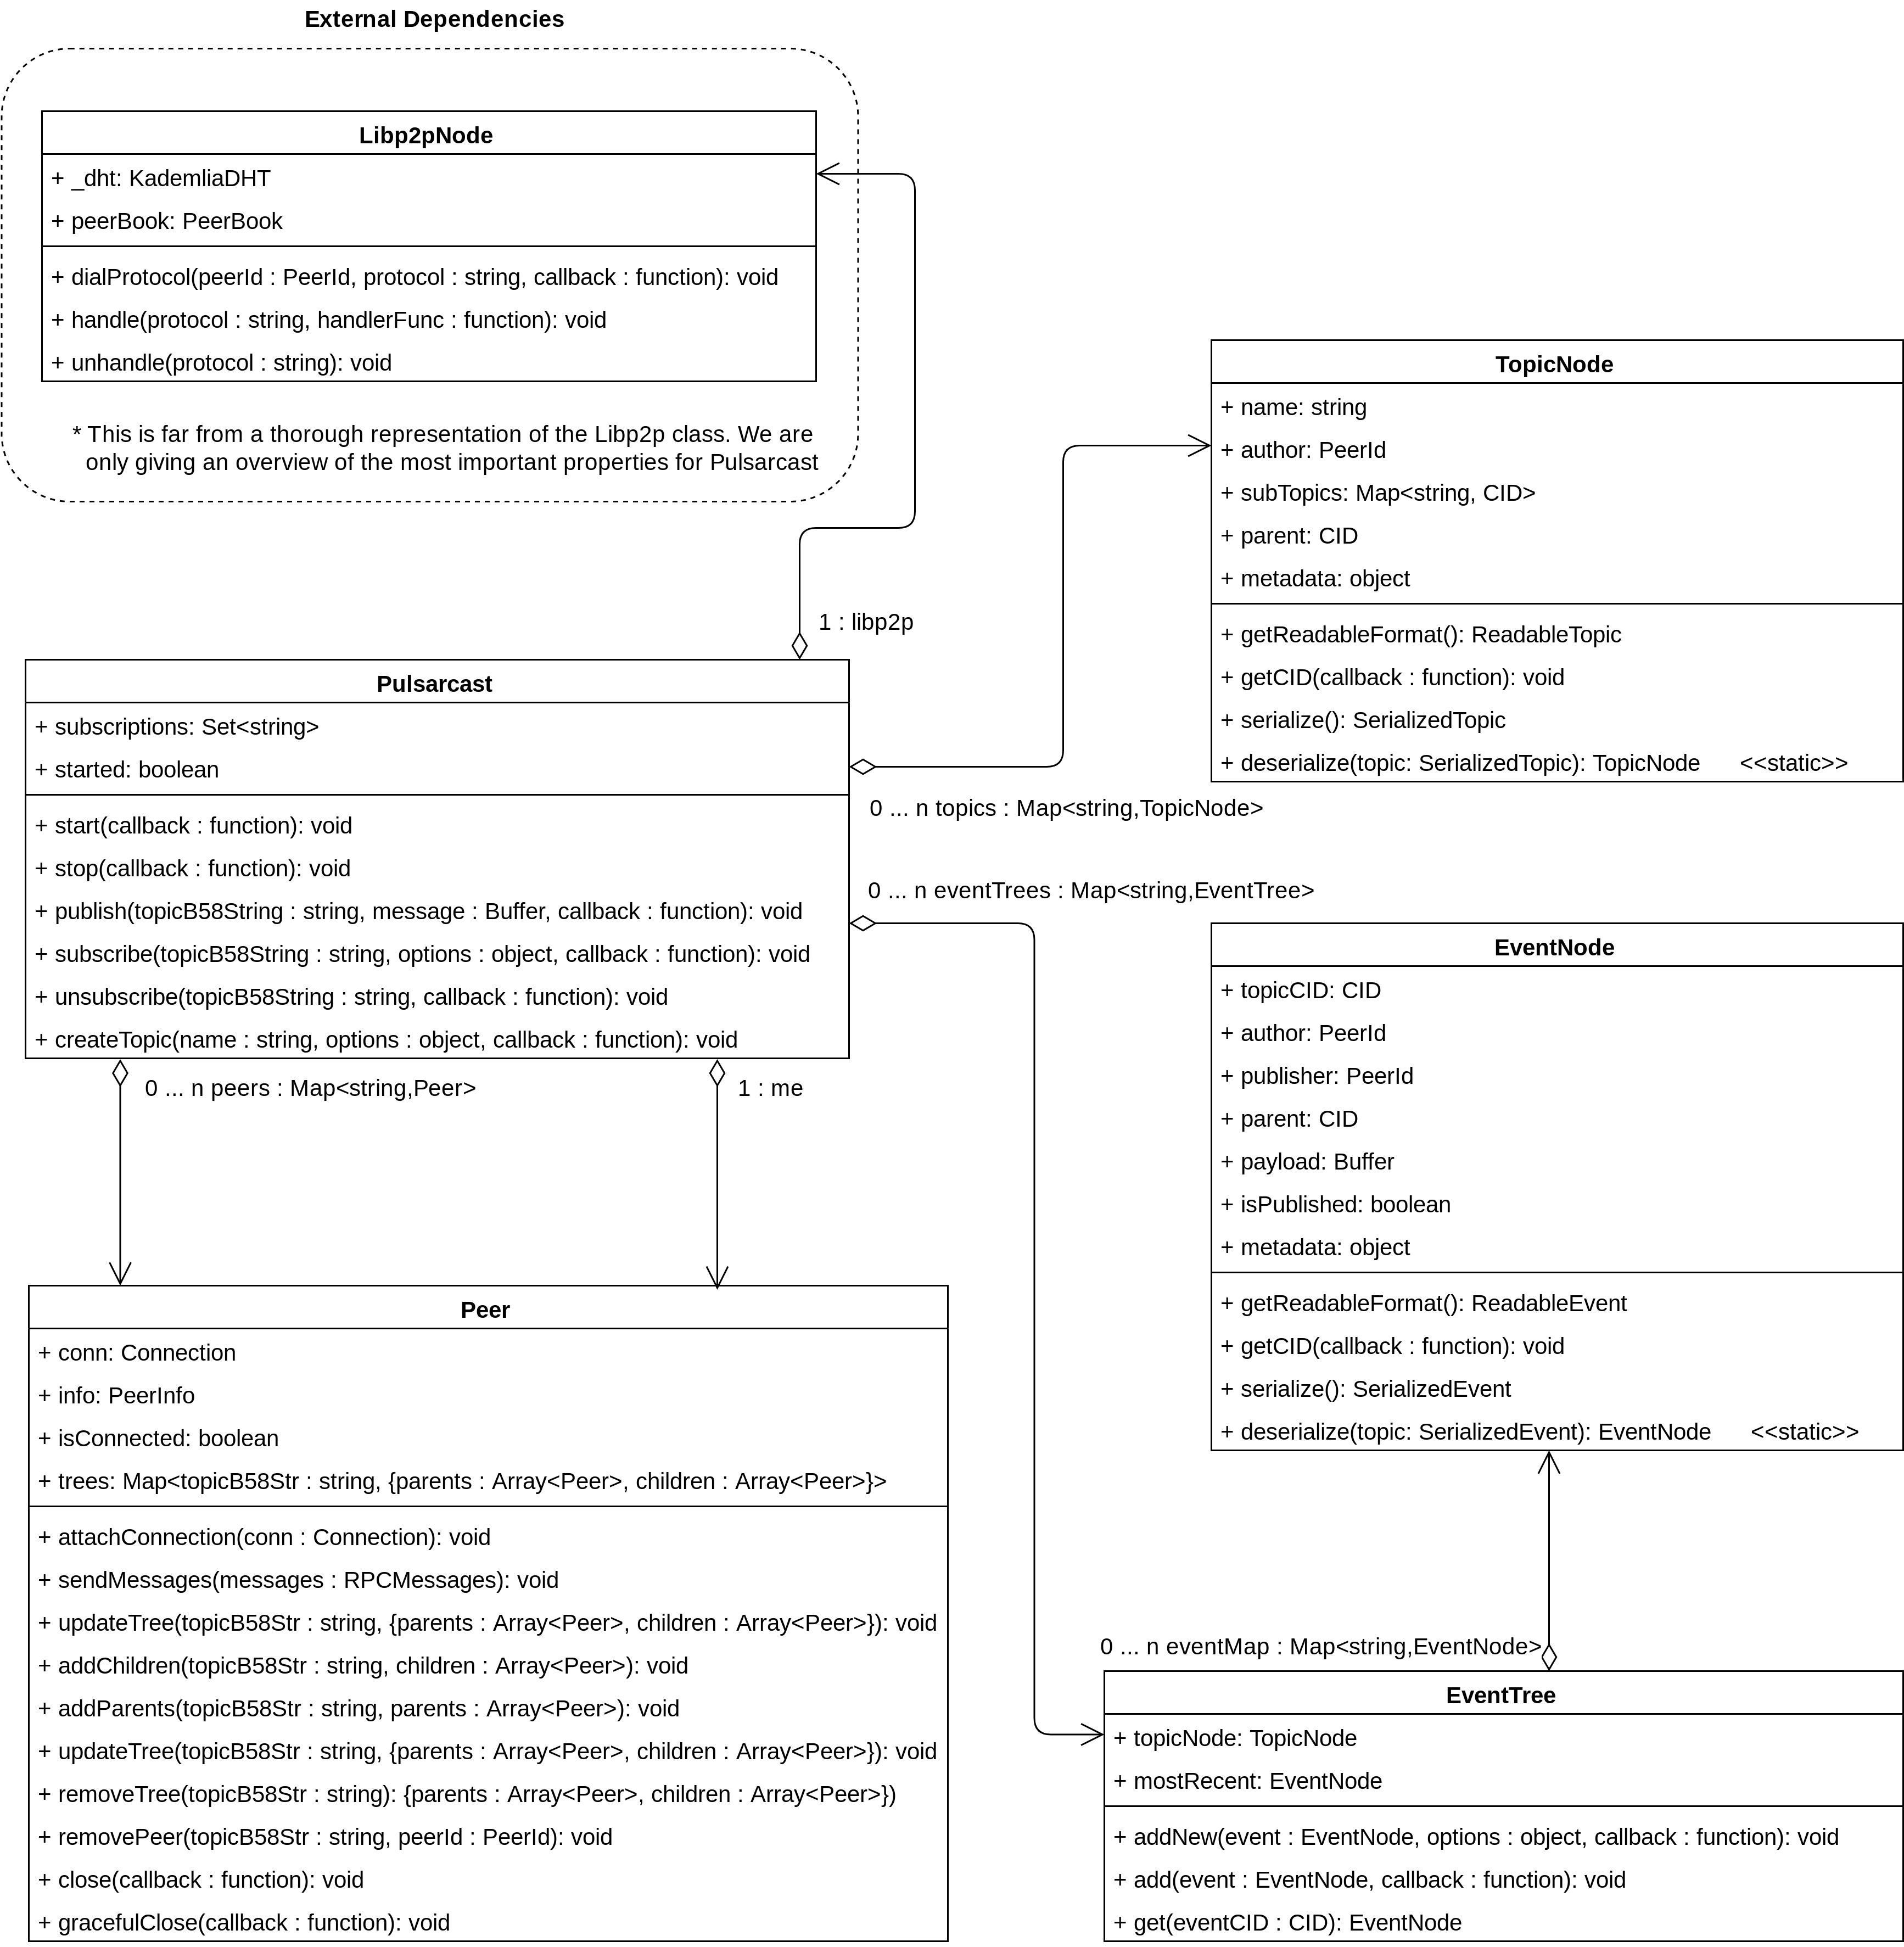
\includegraphics[width=1\textwidth]{img/uml-pulsarcast.png}
  \caption{UML representation of the classes in our Pulsarcast system}
  \label{fig:pulsarcast-uml}
\end{figure}

\subsection{RPC Handlers}\label{subsec:rpc-handlers}

Joi, allows us to define schemas validation schemas  

TODO

\subsection{Usage}\label{subsec:usage}

TODO

\section{Testbed}\label{testbed}

TODO

\section{Summary}\label{summary}

TODO
